\usepackage{xcolor}
\usepackage{afterpage}
\usepackage{hyperref}
\usepackage{caption}
\usepackage{pifont,mdframed}
\usepackage[bottom]{footmisc}

\makeatletter
\gdef\this@inputfilename{input.txt}
\gdef\this@outputfilename{output.txt}
\makeatother

\newcommand{\inputfile}{\texttt{input.txt}}
\newcommand{\outputfile}{\texttt{output.txt}}

\newenvironment{warning}
  {\par\begin{mdframed}[linewidth=2pt,linecolor=gray]%
    \begin{list}{}{\leftmargin=1cm
                   \labelwidth=\leftmargin}\item[\Large\ding{43}]}
  {\end{list}\end{mdframed}\par}

  Grazie ad una recente ricerca che ha confermato l'esistenza delle onde gravitazionali, sempre più persone si stanno interessando allo spazio. Purtroppo però, lo spazio è ancora una realtà poco accessibile alle persone comuni. Sebbene sia un po' demoralizzato da questo fatto, William è convinto che sia possibile sfruttare la recente attenzione mediatica delle onde gravitazionali per pubblicizzare un business: ha deciso infatti di aprire una startup di viaggi interstellari.

  C'è da dire però che, a parte il \emph{Sole} che è la stella a noi più vicina, le altre stelle sono piuttosto distanti. \emph{Proxima Centauri}, la ``seconda stella più vicina'', dista dal Sole ben $4.24$ anni luce: questo vuol dire che sarebbero necessari più di quattro anni per raggiungere questa stella! (supponendo di poter viaggiare alla velocità della luce).

  \begin{figure}[h]
    \centering
    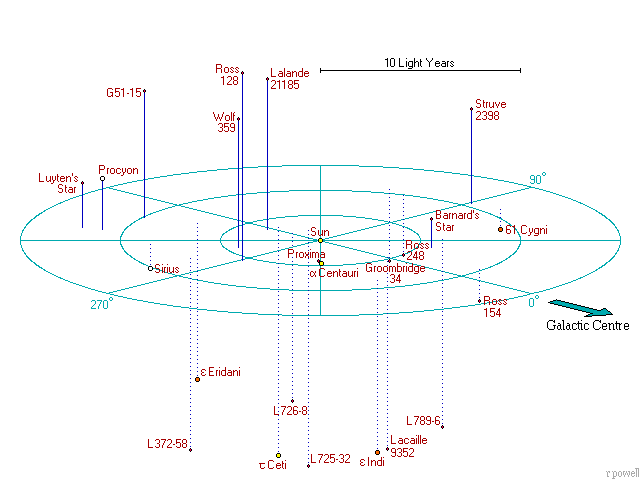
\includegraphics[width=0.8\textwidth]{12ly.png}
    \caption*{Le $33$ stelle che distano al massimo $12.5$ anni luce dal Sole \\ \scriptsize (Richard Powell \href{http://creativecommons.org/licenses/by-sa/2.5}{CC BY-SA 2.5} via Wikimedia Commons)}
  \end{figure}

  William pensa di riuscire a costruire un'astronave in grado di viaggiare alla velocità della luce (ha trovato \href{https://www.youtube.com/watch?v=dQw4w9WgXcQ}{un tutorial su YouTube} che gli sembra piuttosto convincente) e ha perciò acquistato un telescopio per tracciare una mappa 3D della Via Lattea. Ogni stella è indicata nella mappa 3D mediante un punto $(x, y, z)$ dello spazio. Il Sole è sempre presente nella mappa ed è sempre identificato dal punto $(0, 0, 0)$.

  Scrivi un programma che data la mappa stellare sia in grado di rispondere a $Q$ query: ogni query fornisce un numero intero $D$ e chiede quante sono le stelle raggiungibili avendo a disposizione $D$ anni di viaggio.

\Implementation
Dovrai sottoporre esattamente un file con estensione \texttt{.c}, \texttt{.cpp} o \texttt{.pas}.

\begin{warning}
Tra gli allegati a questo task troverai un template (\texttt{annoluce.c}, \texttt{annoluce.cpp}, \texttt{annoluce.pas}) con un esempio di implementazione da completare.
\end{warning}

Se sceglierai di utilizzare il template, dovrai implementare le seguenti funzioni:
\begin{center}\begin{tabularx}{\textwidth}{|c|X|}
\hline
C/C++  & \begin{tabular}[x]{@{}@{}}\verb|void mappatura(int N, int X[], int Y[], int Z[]);|\\ \verb|int query(int D);|\end{tabular}\\
\hline
Pascal & \begin{tabular}[x]{@{}@{}}\verb|procedure mappatura(N: longint; var X, Y, Z: array of longint);|\\ \verb|function query(D: longint) : longint;|\end{tabular}\\
\hline
\end{tabularx}\end{center}
In cui:
\begin{itemize}[nolistsep]
  \item L'intero $N$ rappresenta il numero di stelle nella mappa.
  \item Gli array \texttt{X}, \texttt{Y} e \texttt{Z}, indicizzati da $0$ a $N-1$, contengono le coordinate delle $N$ stelle. In particolare la stella $i$-esima si trova nelle coordinate (\texttt{X[i]}, \texttt{Y[i]}, \texttt{Z[i]}).
  \item La funzione \texttt{mappatura} verrà richiamata una sola volta all'inizio del programma.
  \item Ogni chiamata alla funzione \texttt{query(D)} dovrà restituire il numero di stelle che distano al massimo $D$ anni luce dal Sole.
\end{itemize}

\InputFile
Il file \inputfile{} è composto da $N+Q+2$ righe. La prima riga contiene l'unico intero $N$. Le successive $N$ righe contengono le coordinate $X_i, Y_i, Z_i$ dell'$i$-esima stella, separate da spazio. La successiva riga contiene l'unico intero $Q$. Le successive $Q$ righe contengono i valori di $D$ delle relative query.

\OutputFile
Il file \outputfile{} è composto da $Q$ righe contenente un intero ciascuna: la risposta alla relativa query.

% Assunzioni
\Constraints
\begin{itemize}[nolistsep, itemsep=2mm]
  \item $1 \le N, Q \le 100\,000$.
  \item $0 \le X_i, Y_i, Z_i < 2^{30}$ per ogni $i=0\ldots N-1$.
  \item L'unità degli assi $x, y, z$ è l'anno luce.
  \item $0 \le D < 2^{31}$ per ogni chiamata a \texttt{query(D)}.
  \item Il valore $D$ è espresso in anni luce.
\end{itemize}

\Scoring
Il tuo programma verrà testato su diversi test case raggruppati in subtask.
Per ottenere il punteggio relativo ad un subtask, è necessario risolvere
correttamente tutti i test relativi ad esso.

\pagebreak
\begin{itemize}[nolistsep,itemsep=2mm]
  \item \textbf{\makebox[2cm][l]{Subtask 1} [10 punti]}: Casi d'esempio.
  \item \textbf{\makebox[2cm][l]{Subtask 2} [20 punti]}: $\mathtt{Y[i]} = \mathtt{Z[i]} = 0$ per ogni $i$. Invece che nello spazio tridimensionale, le stelle sono tutte su una retta!
  \item \textbf{\makebox[2cm][l]{Subtask 3} [20 punti]}: $\mathtt{Z[i]} = 0$ per ogni $i$. Invece che nello spazio tridimensionale, siamo su un piano bidimensionale!
  \item \textbf{\makebox[2cm][l]{Subtask 4} [10 punti]}: $N, Q, D \le 10$.
  \item \textbf{\makebox[2cm][l]{Subtask 5} [10 punti]}: $N \le 100$; $D < 10\,000$.
  \item \textbf{\makebox[2cm][l]{Subtask 6} [10 punti]}: $Q \le 100$; $D < 10\,000$.
  \item \textbf{\makebox[2cm][l]{Subtask 7} [20 punti]}: Nessuna limitazione specifica.
\end{itemize}

% Esempi


\Examples
\begin{example}
\exmpfile{annoluce.input0.txt}{annoluce.output0.txt}%
\exmpfile{annoluce.input1.txt}{annoluce.output1.txt}%
\end{example}


\Explanation
Nel \textbf{primo caso di esempio}, le $3$ stelle distano dal sole rispettivamente: $0$ anni luce, $\sqrt{3}$ anni luce e $2\sqrt{3}$ anni luce. \\[2mm]
Nel \textbf{secondo caso di esempio}, le $5$ stelle distano dal sole rispettivamente: $\sqrt{14}$ anni luce, $\sqrt{77}$ anni luce, $0$ anni luce, $9\sqrt{3}$ anni luce e $\sqrt{51}$ anni luce.
